\section{Implementace Time Escape algoritmů}\label{sec:implementace-tea}

Poslední probranou kategorii fraktálních útvarů tvořily tzv. \emph{Juliovy množiny}, u~nichž jsme si jednoduše vysvětlili, že jejich generování probíhá pomocí tzv. \emph{Time Escape algoritmů}\index{Time Escape algoritmus}\index{algoritmus!Time Escape}. Jejich princip lze nastínit následovně: na vstupu zadáme nějakou komplexní polynomiální funkci $f$ a~dále čísla $m\in\N_0$ a~$r\in\R$. Číslo $m$ bude sloužit jako horní hranice počtu iterací, který pro každý bod v~určité omezené oblasti komplexní roviny provedeme (to lze pochopitelně upřesnit, avšak teď to není podstatné). Pokud v~kterékoliv iteraci nastane, že $|f^{\circ k}(z)|>r$, pak bod vyloučíme ze zkoumané množiny. Naopak v~případě, že pro každé $0\leqslant k\leqslant m$ je $|f^{\circ k}(z)|\leqslant r$, prohlásíme, že bod náleží naší aproximaci Juliovy množiny.

\subsection{Aproximace vyplněné Juliovy množiny}\label{subsec:aproximace-vyplnene-juliovy-mnoziny}

Podívejme se na tento algoritmus trochu blíže v~pseudokódu~\ref{alg:generovani-vyplnene-jf}.
\begin{algorithm}
    \KwIn{Komplexní polynomiální funkce $f$, maximální počet iterací $m\in\N_0$, číslo $r\in\R$, konečné množiny $X\subset\langle x_{\text{min}},x_{\text{max}}\rangle$ a~$Y\subset\langle y_{\text{min}},y_{\text{max}}\rangle$}
    $K\gets\emptyset$\;
    \ForEach{\textup{$(a,b)\in X\times Y$}}{
        $z\gets a+b\imag$\;
        $t\gets\id$\;
        \For{$k=0,1,\ldots,m$}{
            $t\gets t\circ f$\;
            \If{$|t(z)|>r$}{
                pokračuj další iterací vnějšího cyklu\;
            }
        }
        $K\gets K\cup\set{z}$\;
    }
    \Return{$K$}\;
    \KwOut{Aproximace vyplněné Juliovy množiny $K(f)$}
    \caption{Generování vyplněné Juliovy množiny při pevném počtu iterací}
    \label{alg:generovani-vyplnene-jf}
\end{algorithm}
Nejspíše nikoho nepřekvapí, že při vyšších hodnotách čísla $m$ obdržíme lepší odhad Juliovy množiny příslušné polynomiální funkci $f$. Avšak vždy je potřeba zvážit náročnost výpočtu.

Znázornění (vyplněné) Juliovy množiny lze provést různými způsoby. Prezentovaný algorimus~\ref{alg:generovani-vyplnene-jf} pouze odhaduje pro každý zvolený bod $z$, zda náleží, či nenáleží množině $J$. Avšak čtenář zajímající se o~tuto partii matematiky již nejspíše viděl poměrně známý způsob vyobrazení těchto množin s~barevným rozlišováním bodů. Tuto záležitost jsme již zmínili ke konci části~\ref{subsec:juliovy-fatouovy-mnoziny}, avšak jeho podstatné aspekty jsou především algoritmické povahy, a~tedy teprve v~této kapitole je více rozvedeme. K~tomu se však dostaneme později.

Praktická implementace Time Escape algoritmů bude podstatně složitější, neboť se musíme vypořádat s~konverzí samotného polynomu a~rovněž vyřešit způsob vzorkování vybrané části komplexní roviny. Dále se budeme držet realizace pomocí třídy (viz ukázka~\ref{prog:konstruktor-tea}).
\begin{program}[h]
\begin{lstlisting}[style=python]
class TEA:
    def __init__(self, width: int, height: int, sequence: str, step: int = 1, escape_radius: int = 2, bounds: tuple, var: str, explore_var: str):
        self._x_count, self._y_count = width // step, height // step
        
        self._iter_counts = [[0 for _ in range(self._x_count)] for _ in range(self._y_count)]
        self._width, self._height = width, height
        self._sequence = sequence
        self._var = var
        self._explore_var = explore_var
        self._total_iterations = 0
        self._escape_radius = escape_radius

        x_min, x_max, y_min, y_max = bounds

        x_vals = [x_min + step * (x_max - x_min) * j / width for j in range(self._x_count + 1)]
        y_vals = [y_min + step * (y_max - y_min) * i / height for i in range(self._y_count + 1)]
        self._complex_grid = [[x + 1j * y for x in x_vals] for y in y_vals]

        self._point_last_values = [[0 for _ in range(self._x_count)] for _ in range(self._y_count)]
\end{lstlisting}
    \caption{Konstruktor třídy \texttt{TEA}}
    \label{prog:konstruktor-tea}
\end{program}
Pojďme si konstruktor~\ref{prog:konstruktor-tea} opět rozebrat.
\begin{itemize}
    \item \texttt{self.\_x\_count} a~\texttt{self.\_y\_count} rozměry obdélníka (coby části komplexní roviny), z~něhož budeme prozkoumávat jednotlivé body. Hodnoty $x$ a $y$ jsou závislé na velikosti kroku \texttt{step}, kterou konstruktor přijímá jako parametr. Tedy např. s~krokem $1$ v~rámci intervalu $\langle-1,2\rangle$ budeme zkoumat celkem 4 body.
    \item V~seznamu \texttt{self.\_iter\_counts} si budeme pro každý bod uchovávat, kolik iterací zadané funkce bylo potřeba, než hodnoty posloupnosti překročily zadanou mez (tedy $|f^{\circ k}(z)|>r$). Ten využijeme především později při přiřazování barev jednotlivým bodům.
    \item \texttt{self.\_sequence} uchovává předpis polynomiální funkce, kterou budeme iterovat, jako řetězec. Předpisy budeme zadávat standardní syntaxí v~Pythonu, tzn.~např. pro Mandelbrotovu množinu, kde $f_c(z)=z^2+c$, bychom předpis napsali
    \begin{center}
        \texttt{z**2 + c}.
    \end{center}
    Levou stranu "\texttt{f(z) =}" pochopitelně psát netřeba.
    \item \texttt{self.\_var} udává, která proměnná v~\texttt{self.\_sequence} je argumentem zadané funkce (typicky \texttt{z}).
    \item \texttt{self.\_explore\_var} uchovává proměnnou, za niž budeme dosazovat hodnoty zkoumaných bodů. Pro Juliovy množiny se typicky jedná přímo o~argument zadané funkce $f$, ale např. pro Mandelbrotovu množinu je to \texttt{c}.
    \item \texttt{self.\_escape\_radius} reprezentuje číslo $r$, tedy hranici absolutní hodnoty čísla $z$, po jejímž překročení prohlásíme posloupnost iterací za divergentní.
    \item Parametr \texttt{bounds} specifikuje část komplexní roviny, z~niž budeme zkoumat vybrané body. Jedná se o~datový typ \texttt{tuple}, v~našem případě uspořádanou čtveřici $(x_{\text{min}},x_{\text{max}},y_{\text{min}},y_{\text{max}})$.
    \item \texttt{self.\_complex\_grid} uchovává všechny body ze zadané části komplexní roviny jako komplexní čísla, tedy v~Pythonu datový typ \texttt{complex}.
    \item Do seznamu \texttt{self.\_point\_last\_values} budeme ukládat hodnoty $f^{\circ k}(z)$ pro zadané $z$, kde $k$ je číslo poslední prozkoumané iterace (tzn. buď jsme u~bodu prozkoumali zadaný maximální počet iterací, nebo výpočet skončil dříve kvůli překročení povolené absolutní hodnoty).
\end{itemize}
Je vidět, že atributů zde máme poměrně hodně. Zkusme si tedy nejdříve vyjasnit, jak bychom mohli pomocí těchto informací implementovat algoritmus pro iterování zadané polynomiální funkce. Již jsme si uvedli asi nejjednodušší možnost v~rámci algoritmu~\ref{alg:generovani-vyplnene-jf}. Jak by se ale situace změnila, kdybychom si uchovávávali počty iterací, které proběhly, než jsme překročili zadanou absolutní hodnotu $r$ nebo dosáhli maximálního počtu $m$? Zaveďme si pole (seznam) $T$, do kterého budeme ukládat počty iterací odpovidající jednotlivům bodům. Podívejme se na algoritmus~\ref{alg:generovani-vyplnene-jf-pole}.
\begin{algorithm}[h]
    \KwIn{Komplexní polynomiální funkce $f$, maximální počet iterací $m\in\N_0$, číslo $r\in\R$, konečné množiny $X\subset\langle x_{\text{min}},x_{\text{max}}\rangle$ a~$Y\subset\langle y_{\text{min}},y_{\text{max}}\rangle$}
    $K\gets\emptyset$\;
    Vytvoř prázdné pole $T$\;
    \ForEach{$(x,y)\in X\times Y$}{
        $z\gets x+y\imag$\;
        $t\gets\id$\;
        \For{$k=0,1,\ldots,m$}{
            $t\gets t\circ f$\;
            $T[x,y]\gets k$\;
            \lIf{$|t(z)|>r$}{opusť cyklus}
        }
        \lIf{$T[x,y]=m$}{$K\gets K\cup\set{z}$}
    }
    \Return{$K$}\;
    \KwOut{Aproximace vyplněné Juliovy množiny $K$}
    \caption{Generování vyplněné Juliovy množiny pomocí pole iterací $T$}
    \label{alg:generovani-vyplnene-jf-pole}
\end{algorithm}
Pro implementaci algoritmu~\ref{alg:generovani-vyplnene-jf-pole} si však budeme muset rozmyslet, jak budeme pomocí řetězce s~předpisem pro funkci $f$ (tj. atributu \texttt{self.\_sequence}) počítat její funkční hodnoty. Jistě se nabízí možnost vytvořit funkci pro vyhodnocení obecného matematického výrazu. Ač se jedná o~poměrně hezké programovací cvičení a~čtenář si jej může vyzkoušet, my si poradíme trochu jinak -- funkcí \texttt{eval}. Funkce \texttt{eval} jednoduše vyhodnotí zadaný výraz a~za proměnné dosadí hodnoty podle slovníku poskytnutého v~příslušném parametru či parametrech.

Tím se nám situace podstatně zlehčuje. Implementaci si může čtenář prohlédnout v~ukázce~\ref{prog:generovani-vyplnene-jf-pole}.
\begin{program}[h]
\begin{lstlisting}[style=python]
def iterate(self, iterations: int) -> None:
    for i in range(self._y_count):
        for j in range(self._x_count):
            # Initialize variables
            vars_dict = {self._var: 0, self._explore_var: self._complex_grid[i][j]}

            # Iterate
            for k in range(1, iterations + 1):
                try:
                    # Evaluate the next value in the sequence
                    vars_dict[self._var] = eval(self._sequence, {"math": math}, vars_dict)

                    # Check for escape condition
                    self._iter_counts[i][j] = k
                    if abs(vars_dict[self._var]) > self._escape_radius:
                        break
                except OverflowError:
                    self._iter_counts[i][j] = k
                    break
            
            self.point_last_values[i][j] = vars_dict[self._var]
\end{lstlisting}
    \caption{Implementace algoritmu~\ref{alg:generovani-vyplnene-jf-pole}}
    \label{prog:generovani-vyplnene-jf-pole}
\end{program}

\subsection{Aproximace Juliovy množiny}\label{subsec:aproximace-juliovy-mnoziny}

S množinou $\filledinjulia(f)$ se rovněž pojí i~její hranice $\boundary{\filledinjulia(f)}$. Co kdybychom chtěli vykreslit pouze hraniční body? Otázka se příliš nevzdaluje té původní, akorát je navíc potřeba o~každém bodu $\filledinjulia(f)$ rozhodnout, zda je hraniční, či nikoliv\footnote{Všimněte si, že zde se nám náramně hodí výsledek z~věty~\ref{thm:vztah-kf-a-jf}, specificky bod~\ref{thm:jf-podmnozina-kf}, kde jsme dokázali, že $\julia(f)\subseteq\filledinjulia(f)$. Náš návrh je tedy v~tomto ohledu oprávněný.}. Přitom myšlenka řešení se vůbec příliš vzdaluje matematickému pojetí hranice. Tu jsme si definovali pro libovolnou množinu $M$ jako množinu takových bodů, které ve svém libovolně malém okolí obsahují alespoň jeden bod, který $M$ náleží a~alespoň jeden, který jí nenáleží. Toho bychom však mohli využít. Stačí zkontrolovat všechny sousední body pro každé $z\in\filledinjulia(f)$, zda alespoň jeden z~nich nenáleží $\fatou(f)$. Pokud ano, pak $z$ prohlásíme za hraniční bod (viz obrázek~\ref{fig:hranicni-bod}).
\begin{figure}[h]
    \centering
    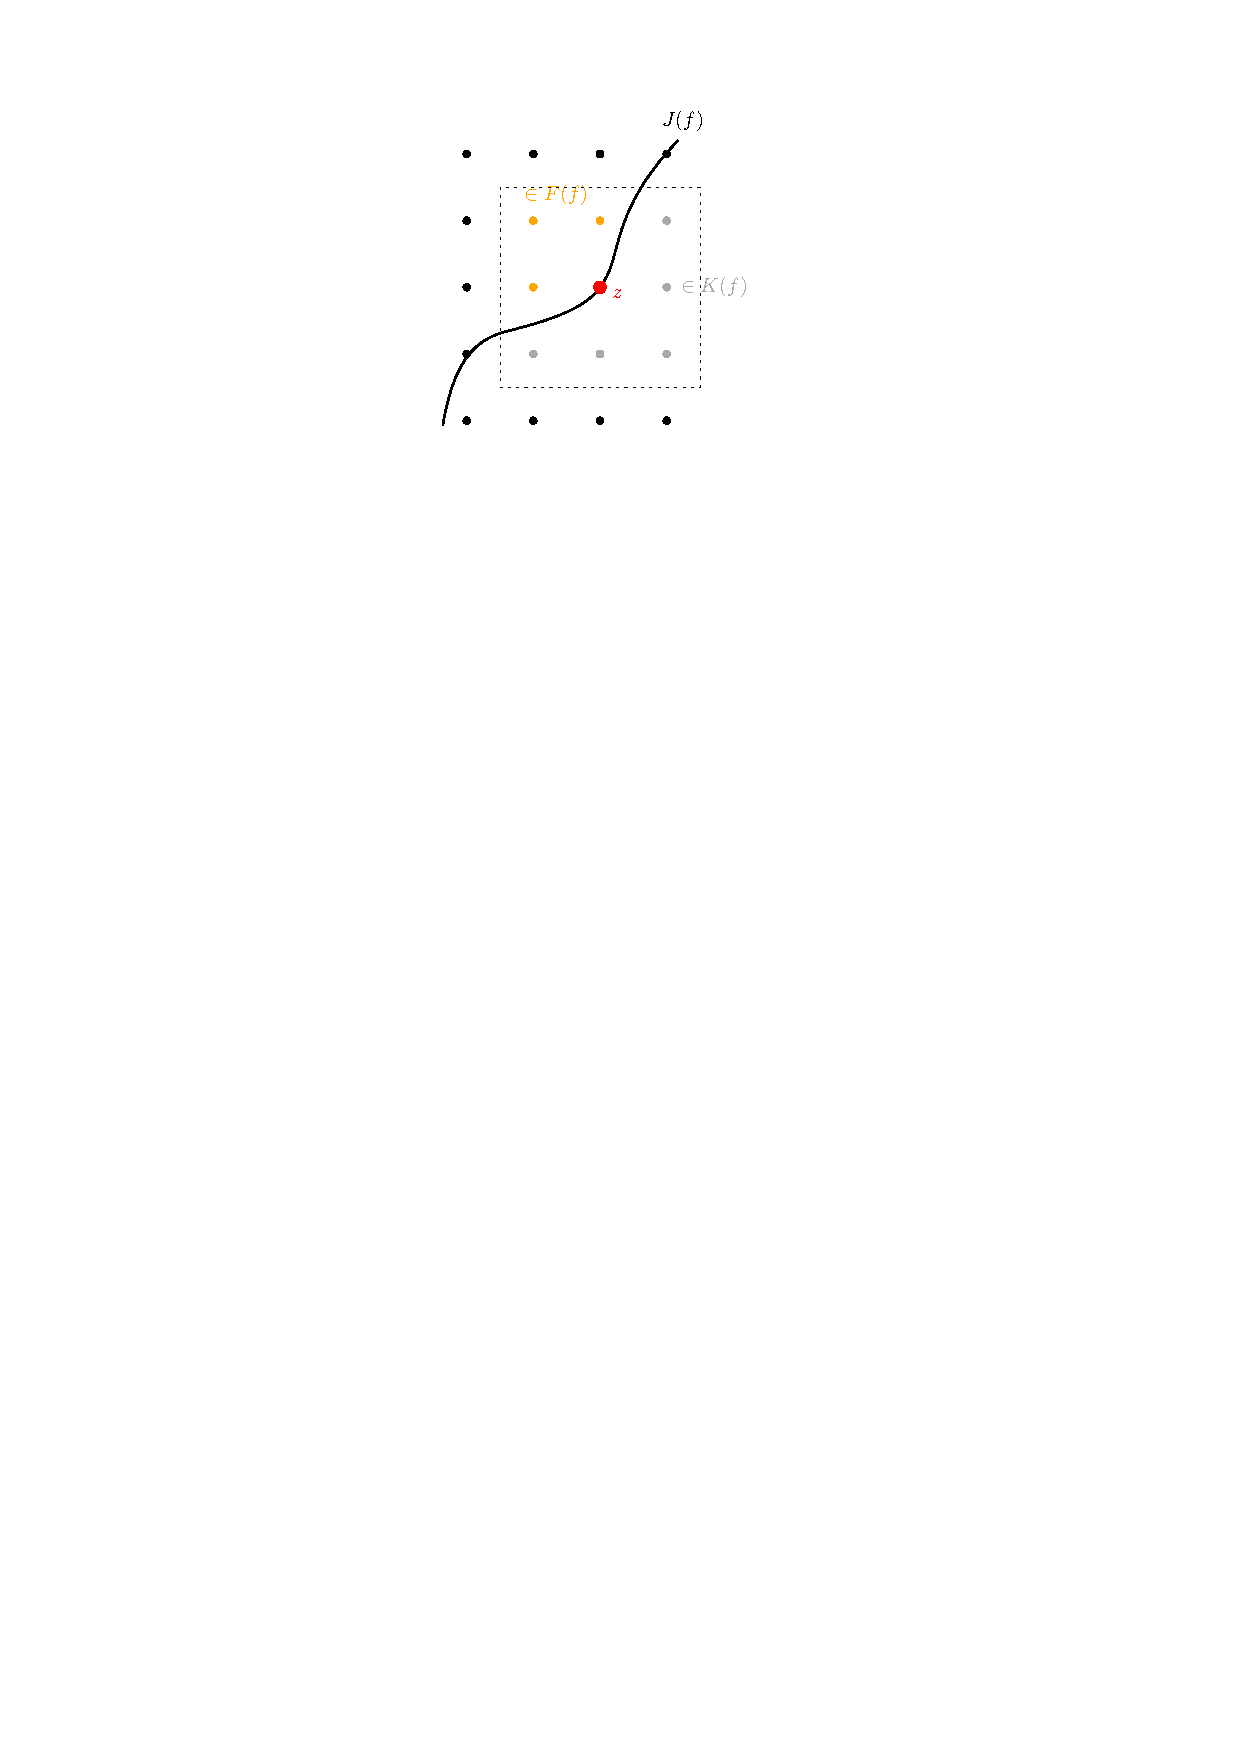
\includegraphics{ch05-hranicni-bod.pdf}
    \caption{Ilustrace hraničního bodu}
    \label{fig:hranicni-bod}
\end{figure}

Na základě této ideje si lze domyslet postup při generování hranice. Pracujeme opět s~předpokladem, že oblast komplexní roviny představuje diskrétní množinu bodů, které tvoří mřížku (tedy každá dvojice sousedních bodů má stejnou vzdálenost). 
\begin{algorithm}[h]
    \KwIn{Komplexní polynomiální funkce $f$, konečné množiny $X\subset\langle x_{\text{min}},x_{\text{max}}\rangle$ a~$Y\subset\langle y_{\text{min}},y_{\text{max}}\rangle$}
    $J\gets\emptyset$\;
    \ForEach{$(x,y)\in X\times Y$}{
        $z\gets x+y\imag$\;
        \If{\textup{existují sousední body $w\in K(f)$ a~$w^\prime\in F(f)$ bodu $z$}}{
            $J\gets J\cup\set{z}$\;
        }
    }
    \Return{$J$}\;
    \KwOut{Aproximace Juliovy množiny $J$}
    \caption{Generování Juliovy množiny $J$}
    \label{alg:generovani-jf}
\end{algorithm}
\begin{program}
\begin{lstlisting}[style=python]
h_px = len(iter_counts)
w_px = len(iter_counts[0])

# List od inner points
inside = [
    [iter_counts[y][x] == max_iterations for x in range(w_px)]
    for y in range(h_px)
]

# Determine boundary points
boundary_mask = [[False]*w_px for _ in range(h_px)]
for y in range(h_px):
    for x in range(w_px):
        if inside[y][x]:
            for dx, dy in ((1,0),(-1,0),(0,1),(0,-1)):
                nx, ny = x+dx, y+dy
                if 0 <= nx < w_px and 0 <= ny < h_px:
                    if not inside[ny][nx]:
                        boundary_mask[y][x] = True
                        break
\end{lstlisting}
    \caption{Implementace algoritmu~\ref{alg:generovani-jf}}
    \label{prog:generovani-jf}
\end{program}

\subsection{Přiřazování barev}\label{subsec:prirazovani-barev}

Jako poslední nás čekají barvy a~jejich přiřazování jednotlivým bodům. Již jsme měli možnost vidět několik příkladů obrázků s~fraktály, v~nichž byly body barevně zvýrazněny. Zhruba bychom mohli říci, že čím blíž se bod nachází hranici útvaru, tím "výraznější" je jeho barva.

\subsubsection{Stručně k~barevnému modelu HSV}

Ukážeme si zde dvojici základních možností, jak lze přiřazovat barvy daným bodům. K~tomu však budeme potřebovat pracovat s~barevným modelem \emph{HSV (Hue, Saturation, Value)}\index{HSV}\index{barevný model}\index{model!barevný}\index{barevný model HSV}. S~prominutím si zde opět odpustíme delší vysvětlování a~budeme předpokládat, že se čtenář již s~modelem HSV někdy setkal (podobně jako např. s~RGB nebo s~CMYK používaným u~tiskáren). Avšak základem, jak název napovídá, je trojice následujících složek:
\begin{itemize}
    \item \textbf{hue} (česky \emph{odstín}),
    \item \textbf{saturation} (česky \emph{saturace}, nebo též \emph{sytost})
    \item a~\textbf{value} reprezentující hodnotu jasu (tj. podílu bílé barvy).
\end{itemize}
Celkově tento model vychází přímo z~vnímání barev lidským okem. Různé možnosti znázornění HSV modelu si lze prohlédnout na obrázcích~\ref{subfig:hsv-valcova-reprezentace} a~\ref{subfig:hsv-kuzelova-reprezentace}.
\begin{figure}[h]
    \centering
    \begin{subfigure}{0.45\textwidth}
        \centering
        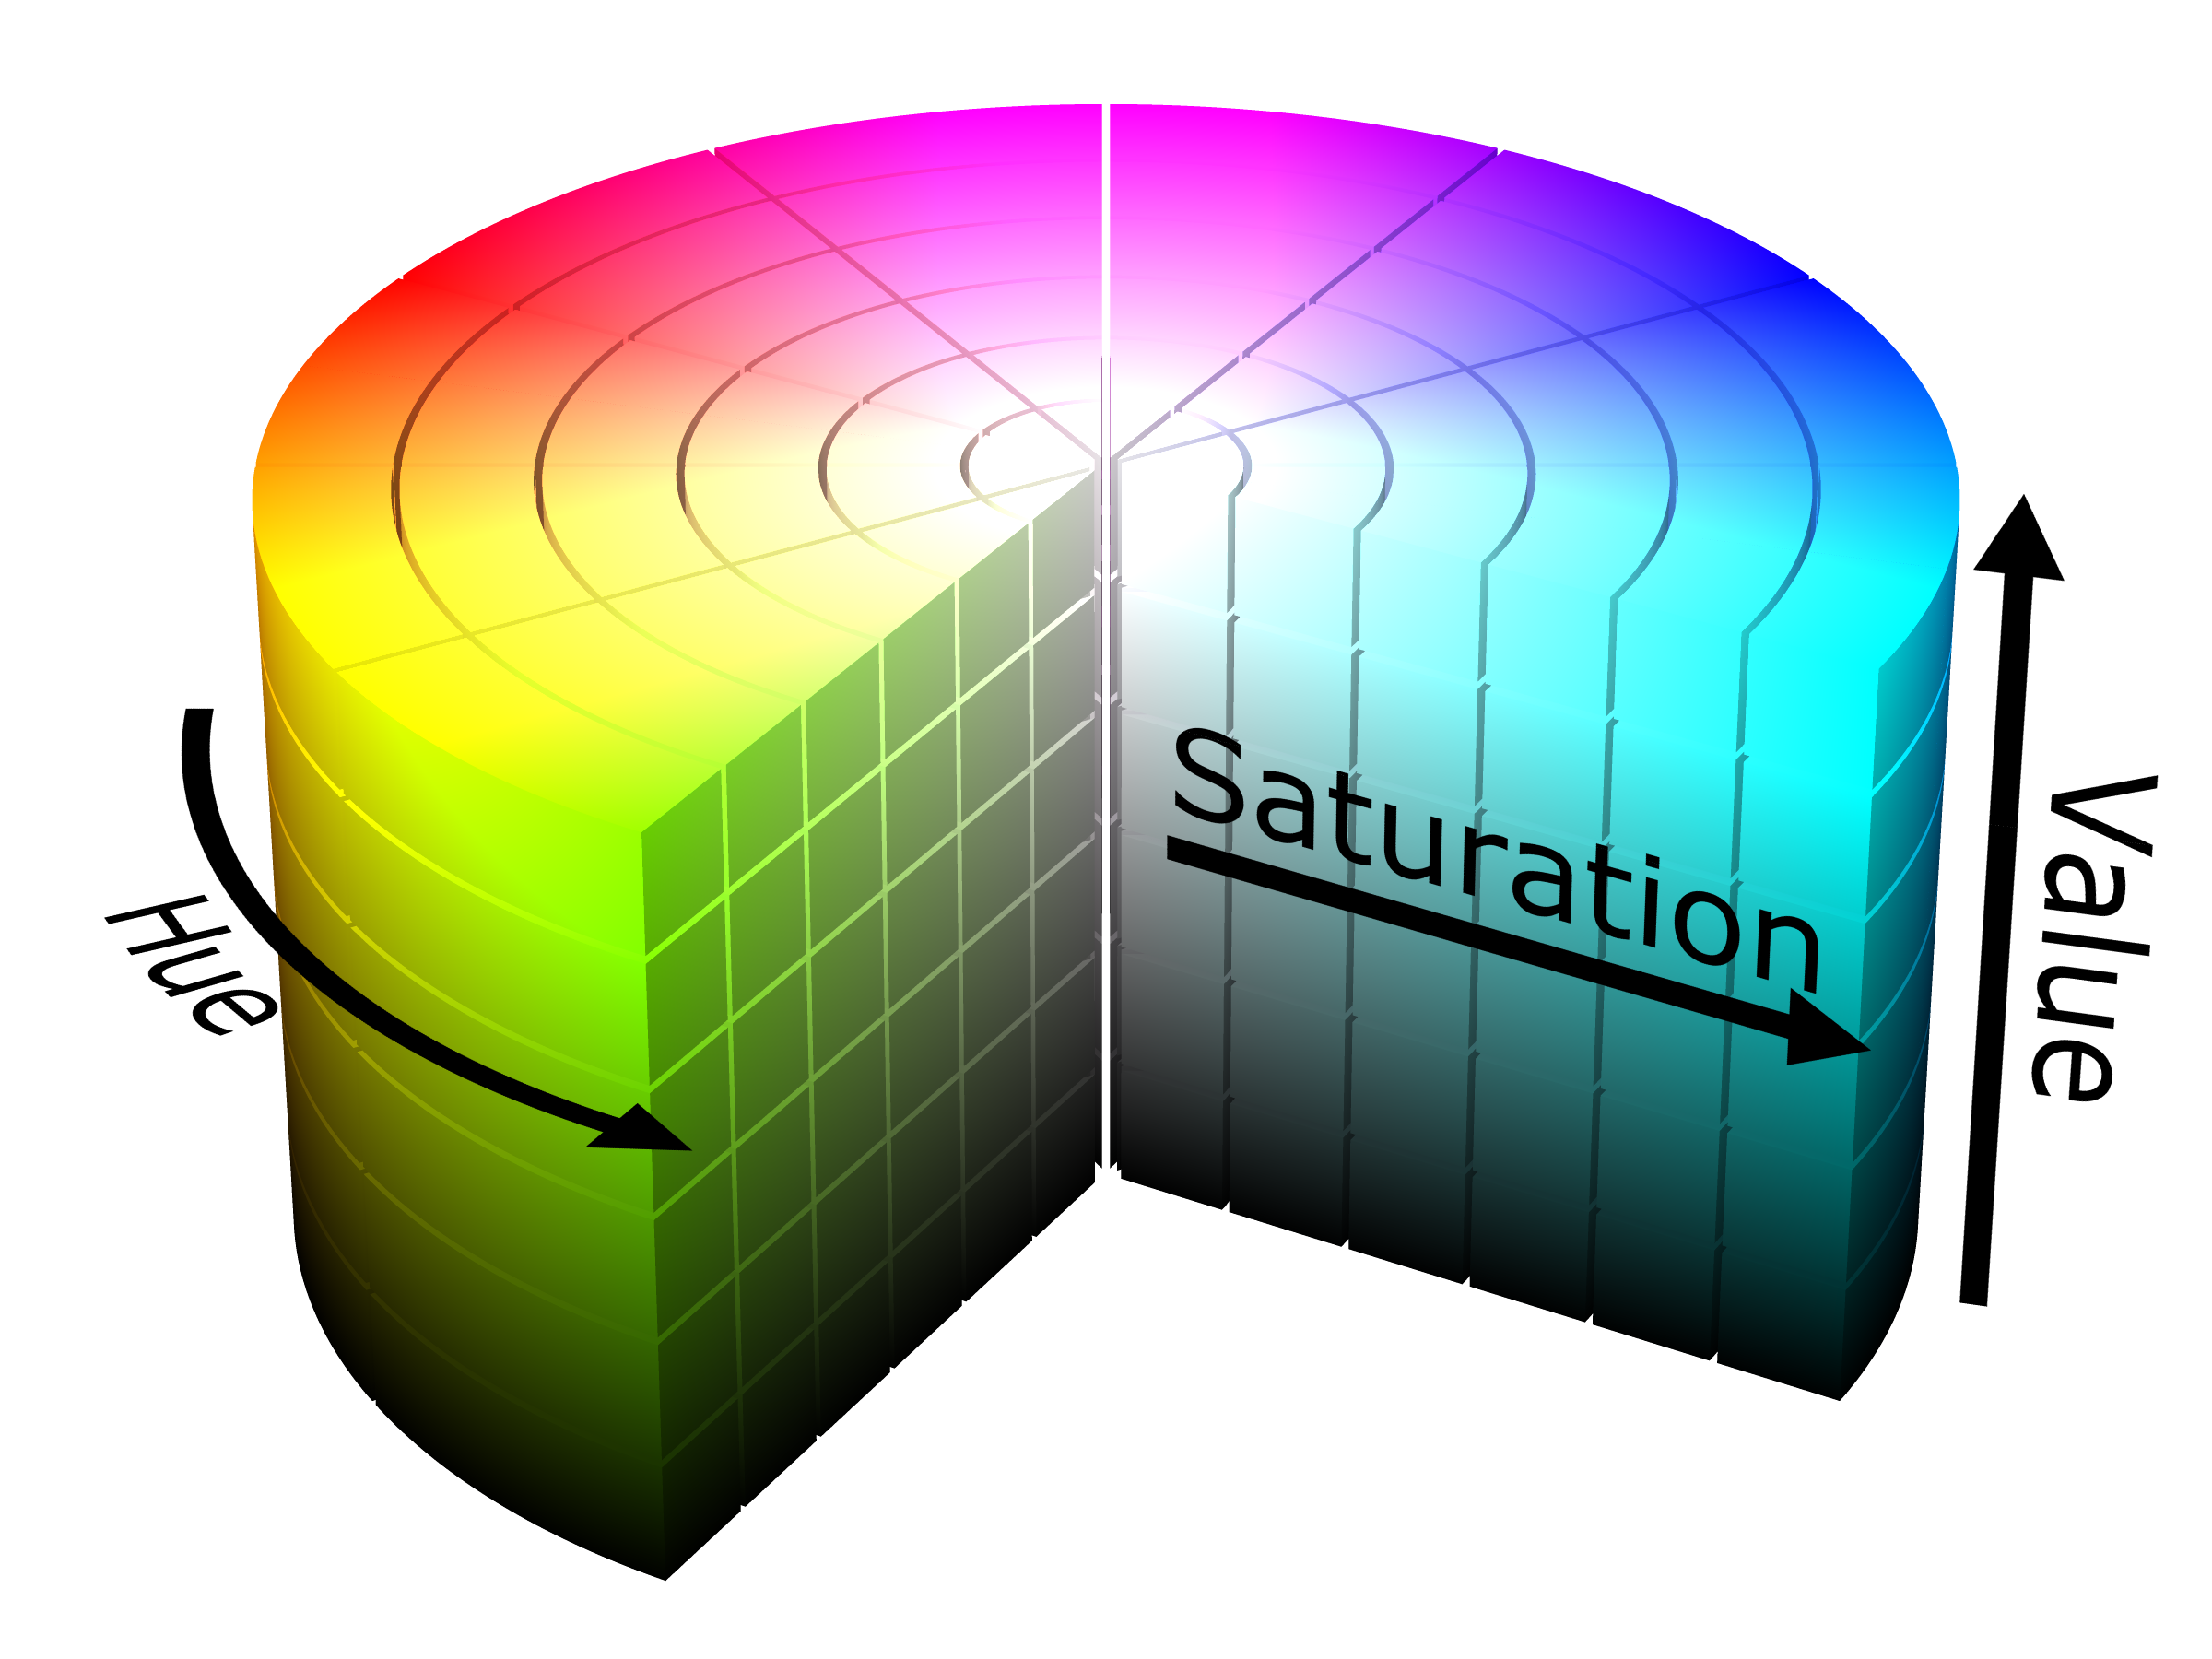
\includegraphics[width=\textwidth]{ch05-HSV_color_solid_cylinder.png}
        \caption{Válcová reprezentace}
        \label{subfig:hsv-valcova-reprezentace}
    \end{subfigure}
    \qquad
    \begin{subfigure}{0.45\textwidth}
        \centering
        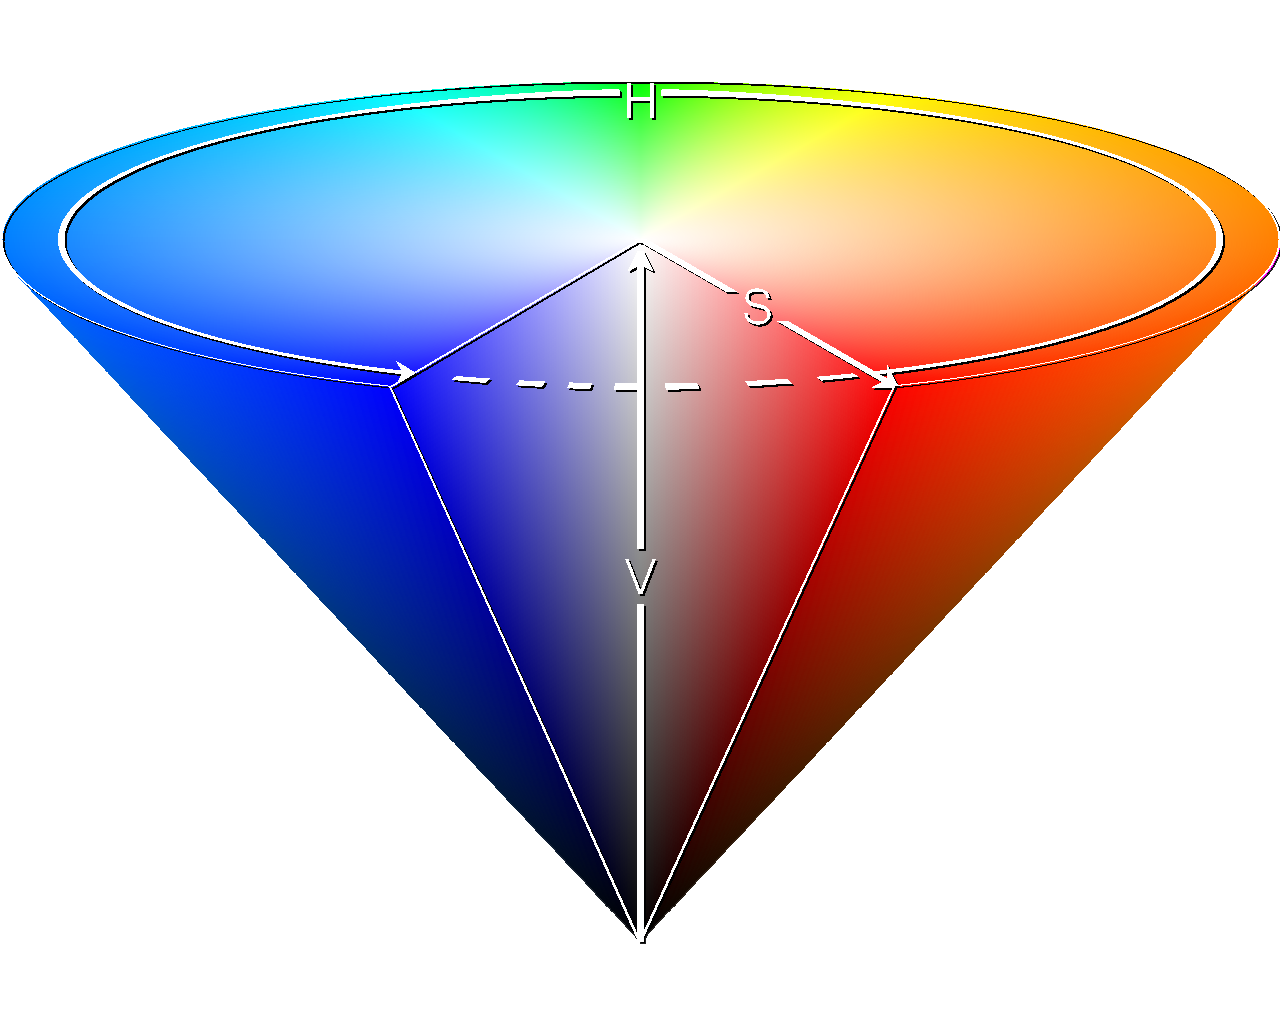
\includegraphics[width=\textwidth]{ch05-HSV_cone.png}
        \caption{Kuželová reprezentace}
        \label{subfig:hsv-kuzelova-reprezentace}
    \end{subfigure}
    \caption[Grafické znázornění HSV modelu]{Grafické znázornění HSV modelu (Převzato z~Wikipedia Commons, viz \href{https://cs.wikipedia.org/wiki/HSV}{\texttt{\textit{odkaz}}})}
    \label{fig:hsv}
\end{figure}

Existují pochopitelně metody pro převody mezi jednotlivými barevnými modely, ty však pro nás zde nejsou relevantní. Jednotlivé barvy budeme reprezentovat jako uspořádané trojice $(H,S,V)$, kde $0\leqslant H,S,V\leqslant 1$.

\subsubsection{Lineární interpolace barev}

Patrně nejjednodušším způsobem pro přiřazení barev jednotlivým bodům je tzv. \emph{lineární interpolací}\index{lineární interpolace}\index{interpolace!lineární} odstínu při pevně zvolené saturaci a~jasu. Obecně, jsou-li zadány body v~rovině $(x_0,y_0)$ a~$(x_1,y_1)$, pak lineární intepolace přiřazuje každému $x\in(x_0,x_1)$ souřadnici $y=f(x)$ takovou, že $(x,y)$ leží na spojnici bodů $(x_0,y_0)$ a~$(x_1,y_1)$. Toto lze vyjádřit poměrně jednoduchým vzorcem:
\[f(x)=y_{0}+(x-x_{0}){\frac {y_{1}-y_{0}}{x_{1}-x_{0}}},\]
tedy grafem bude úsečka spojující oba body (za předpokladu, že $x_0\neq x_1$). Pojďme si nyní rozmyslet náš případ. Bodům z~komplexní roviny budeme přiřazovat barvu podle počtu iterací, kterého jsme při výpočtu dosáhli, než posloupnost absolutních hodnot iterací funkce překročila zadanou mez (popř. po dosažení maximálního počtu iterací). Zde mohou tedy nastat celkově dva případy. Počet iterací pro pevně zvolený bod $z$ si označme $k$ a~maximální počet iterací si označme $m$.
\begin{itemize}
    \item Pokud $k<m$, pak přiřadíme bodu $z$ barvu na základě lineární interpolace odstínu, přičemž saturaci a~jas volíme pevně: označme je $S_0,V_0$.
    \item Pokud $k=m$, pak bodu $z$ přiřadíme černou barvu, tedy prohlásíme jej za bod náležící zkoumané vyplněné Juliově množině.
\end{itemize}

Hodnoty odstínu $H$ jsou z~intervalu $\langle H_{\text{min}},H_{\text{max}}\rangle$, přičemž
\[0\leqslant H_{\text{min}},H_{\text{max}}\leqslant 1\]
a hodnoty $k$ jsou z~množiny $\set{0,1,2,\ldots,m}$. Tedy celkový předpis pro lineární interpolaci odstínu bude
\[H=H_{\text{min}}+k\cdot\frac{H_{\text{max}}-H_{\text{min}}}{m},\]
a tudíž pro výslednou barvu bodu $z$ bude platit 
\[(H,S,V)=\begin{cases}
    \left(H_{\text{min}}+k(H_{\text{max}}-H_{\text{min}})/m,S_0,V_0\right) & k<m,\\
    (0,0,0) & k=m.
\end{cases}\]
Pro ukázku viz obrázky~\ref{fig:mandelbrotova-mnozina-lerp-1} a~\ref{fig:mandelbrotova-mnozina-lerp-2} s~hranicí Mandelbrotovy množiny.
\begin{figure}[h]
    \centering
    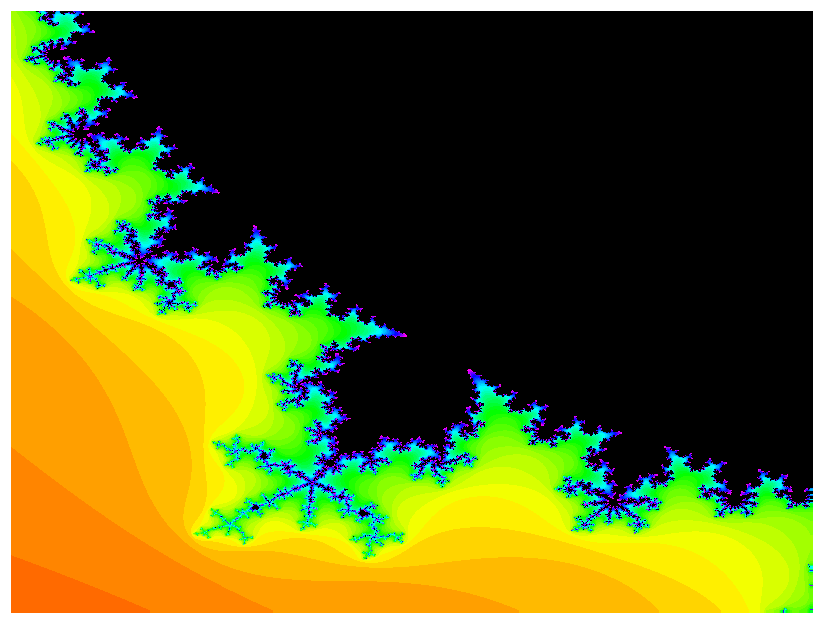
\includegraphics[width=\textwidth]{mandelbrot_set_zoom_1_lerp.png}
    \caption{Mandelbrotova množina pomocí lineární interpolace odstínu pro hodnoty $H_{\text{min}}=0;H_{\text{max}}=0{,}87;S_0=V_0=1;m=50$}
    \label{fig:mandelbrotova-mnozina-lerp-1}
\end{figure}
\begin{figure}[h]
    \centering
    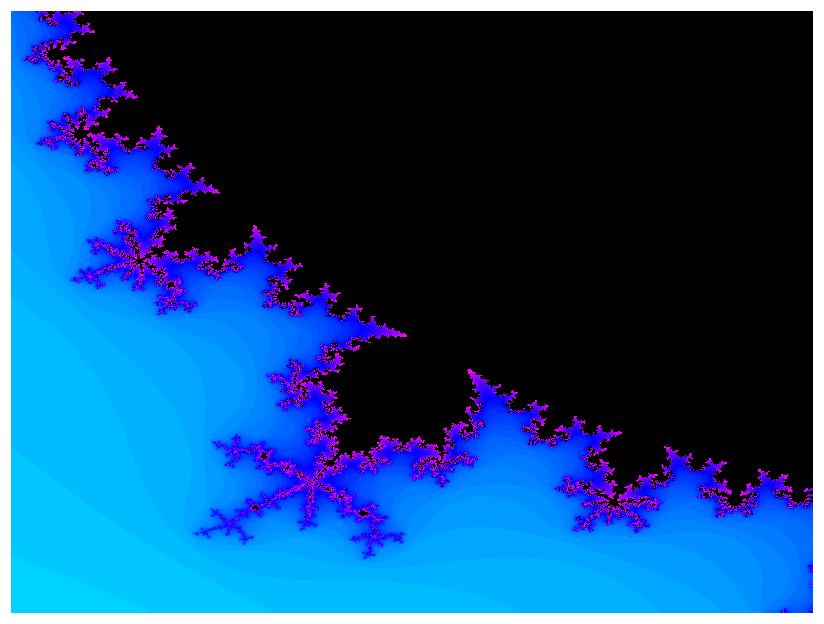
\includegraphics[width=\textwidth]{mandelbrot_set_zoom_1_lerp-2.png}
    \caption{Mandelbrotova množina pomocí lineární interpolace odstínu pro hodnoty $H_{\text{min}}=0{,}5;H_{\text{max}}=0{,}861;S_0=1;V_0=0{,}5;m=50$}
    \label{fig:mandelbrotova-mnozina-lerp-2}
\end{figure}

Pochopitelně stejně jako odstín lze interpolovat i~zbylé dvě složky. Není třeba se omezovat pouze na odstín.
\begin{align*}
    H&=H_{\text{min}}+k\cdot\frac{H_{\text{max}}-H_{\text{min}}}{m},\\
    S&=S_{\text{min}}+k\cdot\frac{S_{\text{max}}-S_{\text{min}}}{m},\\
    V&=V_{\text{min}}+k\cdot\frac{V_{\text{max}}-V_{\text{min}}}{m}.
\end{align*}
Pokud bychom chtěli využít sofistikovanější barvení, mohli bychom též aplikovat obecný interpolační polynom. Ten lze např. určit pomocí tzv. \emph{Lagrangeovy interpolace}\index{interpolace!Lagrangeova}\index{Lagrangeova interpolace}, kdy při známých funkčních hodnonách $f(x_0),f(x_1),\ldots,f(x_n)$ pro navzájem různá $x_0,x_1,\ldots,x_n$ lze sestavit interpolační polynom $L_n(x)$ pomocí vzorce
\[L_n(x)=\sum_{i=0}^{n}f(x_i)\prod_{\substack{0\leqslant j\leqslant n\\j\neq i}}{\frac {x-x_{j}}{x_{i}-x_{j}}}.\]
Lze si všimnout, že takto definovaná funkce $L_n$ prochází všemi zadanými body. Pro libovolné $x_\ell$, kde $0\leqslant\ell\leqslant n$, skutečně platí
\[L_n(x_\ell)=\sum_{i=0}^{n}f(x_i)\prod_{\substack{0\leqslant j\leqslant n\\j\neq i}}{\frac {x_\ell-x_{j}}{x_{i}-x_{j}}}=\sum_{i=0}^{n}f(x_i)\delta_{i\ell}=f(x_\ell),\]
kde $\delta_{ij}$ je Kroneckerovo delta\footnote{Kroneckerovo delta se definuje jako
\[\delta_{ij}=\begin{cases}
    1 & i=j,\\
    0 & i\neq j.
\end{cases}\]
}.

\subsubsection{Hladké zbarvení}

Ačkoliv bychom se s~výsledkem pomocí prosté lineární interpolace (viz obrázky~\ref{fig:mandelbrotova-mnozina-lerp-1} a~\ref{fig:mandelbrotova-mnozina-lerp-2}) mohli spokojit, lze si všimnout, že přechody mezi jednotlivými barvami (coby aproximacemi vyplněné Juliovy množiny pro zvolenou polynomiální funkci) jsou velmi ostré. Je tomu tak z~důvodu, že ze zvolené lineární interpolace vzniká konečná posloupnost hodnot $H$ (funkce tedy není spojitá). Tento problém bychom mohli vyřešit zvýšením maximálního počtu iterací, tedy v~konečném důsledku by mezi barvami nebyly takové rozdíly (pro porovnání s~obrázkem~\ref{fig:mandelbrotova-mnozina-lerp-1} viz obrázek~\ref{fig:mandelbrotova-mnozina-lerp-3}, kde $m=100$).
\begin{figure}[h]
    \centering
    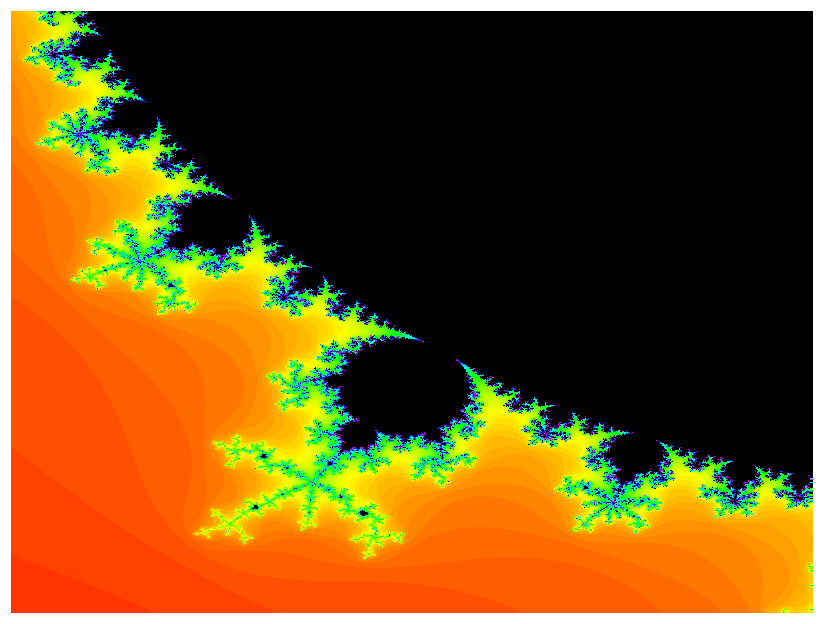
\includegraphics[width=\textwidth]{mandelbrot_set_zoom_1_lerp-3.png}
    \caption{Mandelbrotova množina pomocí lineární interpolace odstínu pro hodnoty $H_{\text{min}}=0;H_{\text{max}}=0{,}87;S_0=V_0=1;m=100$}
    \label{fig:mandelbrotova-mnozina-lerp-3}
\end{figure}
Nicméně zvýšením maximálního počtu iterací se podstatně zvyšuje náročnost výpočtu. Zkusme se tedy místo toho více zaměřit na způsob výpočtu výsledného odstínu. Často se při lineární interpolaci nepoužívá přímo počet iterací $k$, nýbrž číslo
\[k_s=k+\dfrac{\log(\log|f^{\circ k}(z)|)}{\log{2}}.\]
Tento vzorec si zde nebudeme odvozovat, avšak vychází z~tzv. \emph{potenciálové funkce}\index{funkce!potenciálová}\index{potenciálová funkce} definované jako
\[\varphi(z)=\lim_{k\to \infty }{\frac {\log|f^{\circ k}(z)|}{d^{k}}},\]
kde $d=\deg{f}$.

Díky zohlednění absolutní hodnoty $|f^{\circ k}(z)|$ budou přechody mezi barvami již daleko jemnější. To je možno posoudit na obrázku~\ref{fig:mandelbrotova-mnozina-smooth}.
\begin{figure}[h]
    \centering
    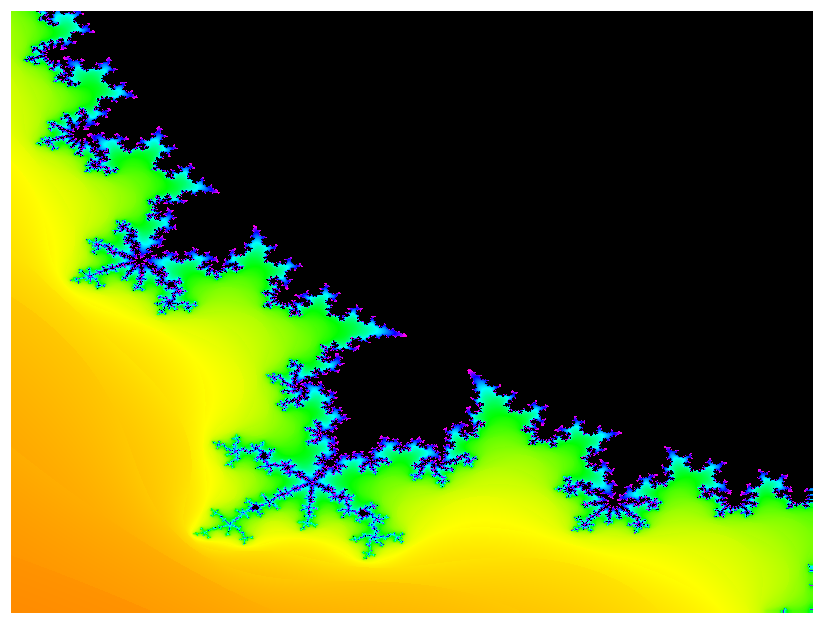
\includegraphics[width=\textwidth]{mandelbrot_set_zoom_1-smooth.png}
    \caption{Mandelbrotova množina pomocí hladkého zbarvení pro hodnoty $H_{\text{min}}=0;H_{\text{max}}=0{,}87;S_0=V_0=1;m=50$}
    \label{fig:mandelbrotova-mnozina-smooth}
\end{figure}